\documentclass[11pt]{article}
\usepackage{amsfonts,amsmath,amssymb,graphicx,url}
\usepackage{fullpage}
\usepackage{amsthm}
\usepackage{epsfig}
\usepackage{graphicx}
\usepackage{wrapfig}
\usepackage{graphicx}
\author{Paavan Kumar}

\title{CSE537  Artificial Intelligence}

\setlength{\oddsidemargin}{.25in}
\setlength{\evensidemargin}{.25in}
\setlength{\textwidth}{6.25in}
\setlength{\topmargin}{-0.4in}
\setlength{\textheight}{8.5in}

\newcommand{\heading}[5]{
   \renewcommand{\thepage}{\arabic{page}}
   \noindent
   \begin{center}
   \framebox{
      \vbox{
    \hbox to 6.2in { {\bf CSE537  Artificial Intelligence}
     	 \hfill #2 }
       \vspace{4mm}
       \hbox to 6.2in { {\Large \hfill #5  \hfill} }
       \vspace{2mm}
       \hbox to 6.2in { { #3 \hfill #4} }
      }
   }
   \end{center}
   \vspace*{4mm}
}

\newcommand{\handout}[3]{\heading{#1}{#2}{\it Paavan Kumar Sirigiri, 109596437  Vivek Pradhan, 109596020         Varsha Paidi, 107677677}{}{#3}}

\setlength{\parindent}{0in}
\setlength{\parskip}{0.1in}



\begin{document}
\handout{1}{\today}{Project 1 report}
\section{Implementation}
{\bf Q 1 to Q4 :}
\\\\ A generic algorithm which returns the list of actions to reach the goal has been implemented for all the search strategies.  Parentnode State   is stored in the dictionary of explored nodes. This information of  parent node states is used to trace the path  from the start state to the goal state. Each search strategy differs in the data structure that is used to maintain the fringe or the frontier. Depth first search uses stack, Breadth first search uses queue, Uniform cost search uses Priority Queue, A star uses Priority Queue with function as their respective data structures. 


{\bf Q5:}

 State has been chosen to be  tuple  of  (position, unvisitedcorners). When the number of unvisited corners is zero, the goal state has been reached.  \\

{\bf Q6:}
 We assume a relaxed problem where there are no walls in the maze. The heuristic for the corners problem is chosen to be  sum of the manhattan distance to the closest  corner from the pacman postion and manhattan distances betwwen the unvisited corners. \\
 
    \begin{tabular}{c c  p{5cm} c  p{5cm}}
  Corners heuristic&=& Manhattan distance to closest corner from the pacman position available &+&  Sum of the manhattan distances betwwen the unvisited corners\\
  \end{tabular}
  
  This heuristic is admissible as it is always  less than the actual cost of collecting all the food by pacman. The heuristic is also consistent because the difference between heuristics for two consecutive states is always less than the actual step cost  between the states.\\

{\bf Q7:}
We assume a relaxed problem where there are no walls in the maze. Food heuristic is taken to be the minimum possible distance that will be traversed by the pacman to collect all the food.  Pacman position is also taken to be as a food dot for calculation of the minimum distance. For the heuristic estimate, we considered the sum of the  maximum vertical difference of the food dots  in each column  of the maze grid . To this, we add  the maximum horizontal distance of the all the food dots in the maze . Also,  we add the vertical  gaps the pacman has to travel   while traversing between one column to the adjacent column.\\

$$ \text{Food heuristic}=  [\sum_{i=1}^{foodGridwidth}  (Ymax_i  - Ymin_i +VerticalGap_i )]     + (Xmax_i   - Xmin_i)  $$ \\ 
\begin{figure}[h!]
 
  \centering
    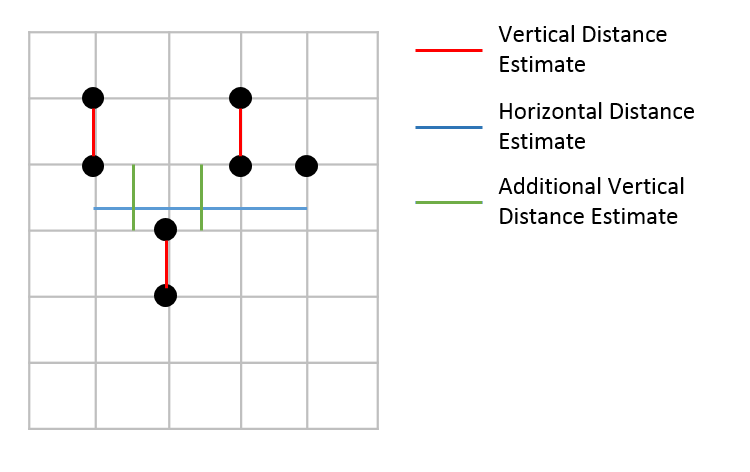
\includegraphics[width=0.8\textwidth]{image.png}
     \caption{Food Grid}
\end{figure}

This heuristic is admissible as it is always  less than the actual cost of collecting all the food by pacman. The heuristic is also consistent because the difference between heuristics for two consecutive states is always less than the actual step cost  between the states.\\

\section{Statistics}

{\bf Q 1 :}
\bgroup\obeylines

{\bf TinyMaze :}
[SearchAgent] using function depthFirstSearch
[SearchAgent] using problem type PositionSearchProblem
Path found with total cost of 10 in 0.0 seconds
Search nodes expanded: 16
Pacman emerges victorious! Score: 500
Average Score: 500.0
Scores:        500
Win Rate:      1/1 (1.00)
Record:        Win
{\bf MediumMaze :}
[SearchAgent] using function depthFirstSearch
[SearchAgent] using problem type PositionSearchProblem
Path found with total cost of 130 in 0.0 seconds
Search nodes expanded: 146
Pacman emerges victorious! Score: 380
Average Score: 380.0
Scores:        380
Win Rate:      1/1 (1.00)
Record:        Win
{\bf BigMaze :}
[SearchAgent] using function depthFirstSearch
[SearchAgent] using problem type PositionSearchProblem
Path found with total cost of 210 in 0.0 seconds
Search nodes expanded: 391
Pacman emerges victorious! Score: 300
Average Score: 300.0
Scores:        300
Win Rate:      1/1 (1.00)
Record:        Win
{\bf Q 2 :}
{\bf MediumMaze :}
[SearchAgent] using function bfs
[SearchAgent] using problem type PositionSearchProblem
Path found with total cost of 68 in 0.0 seconds
Search nodes expanded: 270
Pacman emerges victorious! Score: 442
Average Score: 442.0
Scores:        442
Win Rate:      1/1 (1.00)
Record:        Win
{\bf BigMaze :}
[SearchAgent] using function bfs
[SearchAgent] using problem type PositionSearchProblem
Path found with total cost of 210 in 0.1 seconds
Search nodes expanded: 621
Pacman emerges victorious! Score: 300
Average Score: 300.0
Scores:        300
Win Rate:      1/1 (1.00)
Record:        Win
{\bf Q 3 :}
{\bf MediumMaze :}
[SearchAgent] using function ucs
[SearchAgent] using problem type PositionSearchProblem
Path found with total cost of 68 in 0.0 seconds
Search nodes expanded: 269
Pacman emerges victorious! Score: 442
Average Score: 442.0
Scores:        442
Win Rate:      1/1 (1.00)
Record:        Win
{\bf MediumDottedMaze :}
Path found with total cost of 1 in 0.0 seconds
Search nodes expanded: 187
Pacman emerges victorious! Score: 646
Average Score: 646.0
Scores:        646
Win Rate:      1/1 (1.00)
Record:        Win
{\bf MediumScaryMaze :}
Path found with total cost of 68719479864 in 0.0 seconds
Search nodes expanded: 108
Pacman emerges victorious! Score: 418
Average Score: 418.0
Scores:        418
Win Rate:      1/1 (1.00)
Record:        Win
{\bf Q4 :}
{\bf Manhattan Heuristic :}
[SearchAgent] using function astar and heuristic manhattanHeuristic
[SearchAgent] using problem type PositionSearchProblem
Path found with total cost of 210 in 0.0 seconds
Search nodes expanded: 539
Pacman emerges victorious! Score: 300
Average Score: 300.0
Scores:        300
Win Rate:      1/1 (1.00)
Record:        Win
{\bf Null Heuristic :}
[SearchAgent] using function astar and heuristic nullHeuristic
[SearchAgent] using problem type PositionSearchProblem
Path found with total cost of 210 in 0.1 seconds
Search nodes expanded: 620
Pacman emerges victorious! Score: 300
Average Score: 300.0
Scores:        300
Win Rate:      1/1 (1.00)
Record:        Win
{\bf Q5 :}
{\bf tinyCorners :}
[SearchAgent] using function bfs
[SearchAgent] using problem type CornersProblem
Path found with total cost of 28 in 0.0 seconds
Search nodes expanded: 253
Pacman emerges victorious! Score: 512
Average Score: 512.0
Scores:        512
Win Rate:      1/1 (1.00)
Record:        Win
{\bf mediumCorners :}
[SearchAgent] using function bfs
[SearchAgent] using problem type CornersProblem
Path found with total cost of 106 in 0.4 seconds
Search nodes expanded: 1967
Pacman emerges victorious! Score: 434
Average Score: 434.0
Scores:        434
Win Rate:      1/1 (1.00)
Record:        Win
{\bf Q6 :}

Path found with total cost of 106 in 0.1 seconds
Search nodes expanded: 775
Pacman emerges victorious! Score: 434
Average Score: 434.0
Scores:        434
Win Rate:      1/1 (1.00)
Record:        Win
{\bf Q7 :}
Path found with total cost of 60 in 11.4 seconds
Search nodes expanded: 6850
Pacman emerges victorious! Score: 570
Average Score: 570.0
Scores:        570
Win Rate:      1/1 (1.00)
Record:        Win
\egroup

\section{Critical Analysis}
The following observations and inferences can be made from the statistics.\\
1. In the pacman problem,  Breadth first search has expanded  more nodes than Depth first search  before reaching the goal state  as Depth first search searches deeper nodes faster.\\

2. A-star search finds the goal state by expanding lesser number of nodes if there is a good  heuristic. As observed, in Q4,  Manhattan heuristic expands very less number of nodes(539) compared to null heuristic(620). Hence, choosing a admissible and consistent heuristic that better approximates the actual distance to goal state is crucial.\\

3. For the food heuristic problem, we observed that giving a better approximation of the distance to the goal state drastically reduces the number of expanded nodes. Initially we used the sum of the  maximum vertical difference of the food dots  in each column  of the maze grid  as the  heuristic and were able to expand 13534 nodes. We improved this to 8157 nodes by adding  maximum horizontal distance of the food dots to the heuristic. Further improvement to 6864 nodes has been observed by adding the vertical gap distance the pacman has to travel to reach from one column to the  adjacent column.\\
  We tried to consider the closest food dot to pacman position for the heuristic estimate. Doing this way would have given better approximation of the heuristic  but that was computationally intensive and took more time to expand all the nodes. Therefore we considered pacman also as a food dot. 




\end{document}
